%!TEX root = ../dissertation.tex

% If you do want an image in the colophon:
\begin{figure}[h!]
  \centering
  %\hspace*{-32pt}
  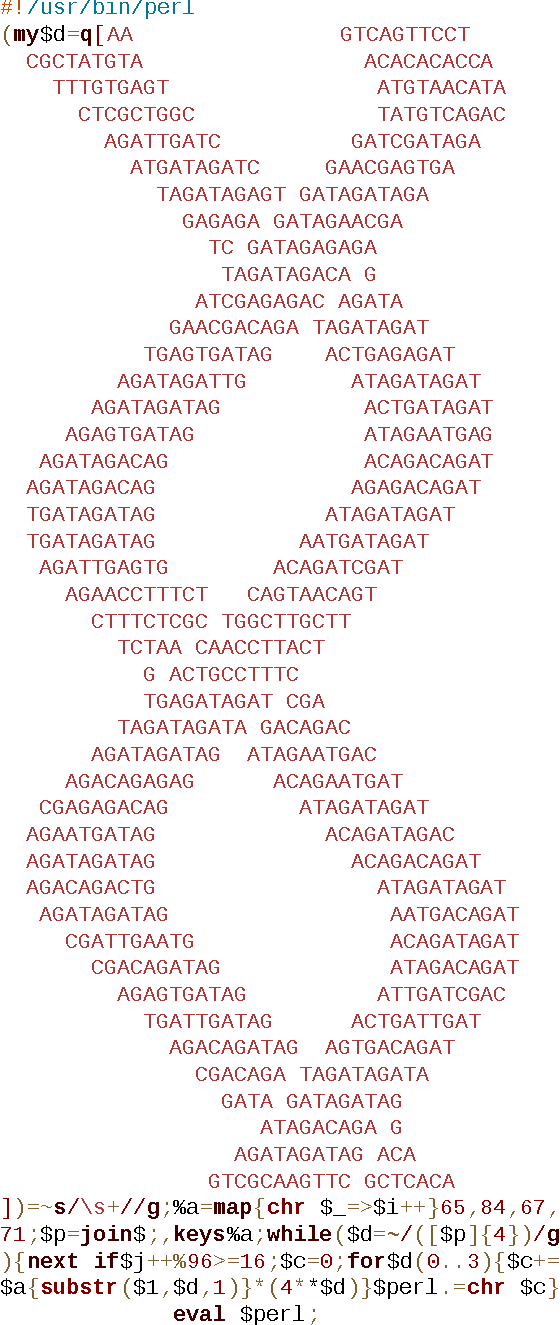
\includegraphics[width=0.5\textwidth]{endmatter/jagh}
\end{figure}

\newpage
% If you don't want an image in the colophon:
% \vspace*{200pt}

\begin{center}
\parbox{200pt}{\lettrine[lines=3,slope=-2pt,nindent=-4pt]{\textcolor{SchoolColor}{T}}{ his thesis was typeset} using \LaTeX, originally developed by Leslie Lamport and based on Donald Knuth's \TeX. The body text is set in 11 point Egenolff-Berner Garamond, a revival of Claude Garamont's humanist typeface. The above illustration is an obfuscated Perl program that prints the text ``Just another genome hacker''. Unfortunately, the source for this program is no longer known to me. A template that can be used to format a PhD dissertation with this look \textit{\&} feel has been released under the permissive \textsc{agpl} license, and can be found online at \href{https://github.com/suchow/Dissertate}{github.com/suchow/Dissertate} or from its lead author, Jordan Suchow, at \href{mailto:suchow@post.harvard.edu}{suchow@post.harvard.edu}.}
\end{center}
